باید یک DFA طراحی کنیم که دو زیررشته‌ی "000" و "111" را نپذیرد. با توجه توضیحات، DFA مورد نظر به این شکل خواهد بود:


\begin{center}
	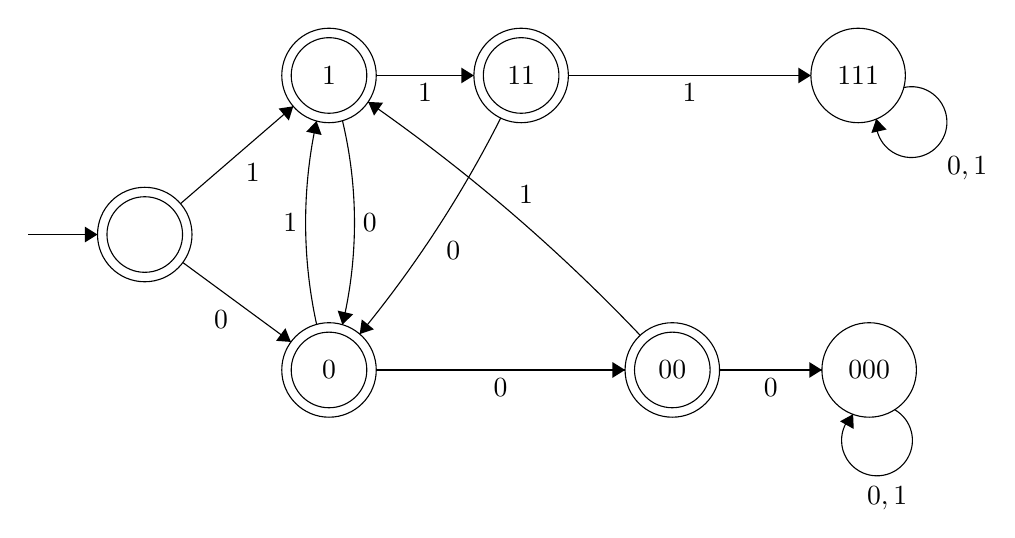
\begin{tikzpicture}[scale=0.2]
		\tikzstyle{every node}+=[inner sep=0pt]
		\draw [black] (13.2,-17.8) circle (3);
		\draw [black] (13.2,-17.8) circle (2.4);
		\draw [black] (24.9,-7.7) circle (3);
		\draw (24.9,-7.7) node {$1$};
		\draw [black] (24.9,-7.7) circle (2.4);
		\draw [black] (24.9,-26.4) circle (3);
		\draw (24.9,-26.4) node {$0$};
		\draw [black] (24.9,-26.4) circle (2.4);
		\draw [black] (37.1,-7.7) circle (3);
		\draw (37.1,-7.7) node {$11$};
		\draw [black] (37.1,-7.7) circle (2.4);
		\draw [black] (46.7,-26.4) circle (3);
		\draw (46.7,-26.4) node {$00$};
		\draw [black] (46.7,-26.4) circle (2.4);
		\draw [black] (59.2,-26.4) circle (3);
		\draw (59.2,-26.4) node {$000$};
		\draw [black] (58.5,-7.7) circle (3);
		\draw (58.5,-7.7) node {$111$};
		\draw [black] (5.8,-17.8) -- (10.2,-17.8);
		\fill [black] (10.2,-17.8) -- (9.4,-17.3) -- (9.4,-18.3);
		\draw [black] (15.47,-15.84) -- (22.63,-9.66);
		\fill [black] (22.63,-9.66) -- (21.7,-9.8) -- (22.35,-10.56);
		\draw (20.06,-13.24) node [below] {$1$};
		\draw [black] (15.62,-19.58) -- (22.48,-24.62);
		\fill [black] (22.48,-24.62) -- (22.13,-23.75) -- (21.54,-24.55);
		\draw (18.05,-22.6) node [below] {$0$};
		\draw [black] (27.9,-7.7) -- (34.1,-7.7);
		\fill [black] (34.1,-7.7) -- (33.3,-7.2) -- (33.3,-8.2);
		\draw (31,-8.2) node [below] {$1$};
		\draw [black] (27.9,-26.4) -- (43.7,-26.4);
		\fill [black] (43.7,-26.4) -- (42.9,-25.9) -- (42.9,-26.9);
		\draw (35.8,-26.9) node [below] {$0$};
		\draw [black] (27.385,-9.38) arc (55.17282:43.58132:112.698);
		\fill [black] (27.39,-9.38) -- (27.76,-10.25) -- (28.33,-9.43);
		\draw (37.41,-15.86) node [above] {$1$};
		\draw [black] (24.113,-23.506) arc (-167.63365:-192.36635:30.147);
		\fill [black] (24.11,-10.59) -- (23.45,-11.27) -- (24.43,-11.48);
		\draw (22.91,-17.05) node [left] {$1$};
		\draw [black] (25.754,-10.574) arc (13.45124:-13.45124:27.838);
		\fill [black] (25.75,-23.53) -- (26.43,-22.86) -- (25.45,-22.63);
		\draw (27.02,-17.05) node [right] {$0$};
		\draw [black] (35.803,-10.405) arc (-26.7821:-39.45928:74.18);
		\fill [black] (26.85,-24.12) -- (27.75,-23.82) -- (26.98,-23.19);
		\draw (32.32,-18.83) node [right] {$0$};
		\draw [black] (49.7,-26.4) -- (56.2,-26.4);
		\fill [black] (56.2,-26.4) -- (55.4,-25.9) -- (55.4,-26.9);
		\draw (52.95,-26.9) node [below] {$0$};
		\draw [black] (60.81,-28.917) arc (60.34019:-227.65981:2.25);
		\draw (60.34,-33.76) node [below] {$0,1$};
		\fill [black] (58.18,-29.21) -- (57.35,-29.66) -- (58.22,-30.15);
		\draw [black] (40.1,-7.7) -- (55.5,-7.7);
		\fill [black] (55.5,-7.7) -- (54.7,-7.2) -- (54.7,-8.2);
		\draw (47.8,-8.2) node [below] {$1$};
		\draw [black] (61.388,-8.469) arc (102.81407:-185.18593:2.25);
		\draw (64.12,-13.6) node [right] {$0,1$};
		\fill [black] (59.65,-10.46) -- (59.34,-11.35) -- (60.31,-11.13);
	\end{tikzpicture}
\end{center}

همانطور که مشخص است، اگر زیررشته‌ی "111" یا "000" مشاهده شود، ماشین داخل Trap می‌افتد و همواره دارای State غیر قابل قبول است.

	


